%%%%%%%%%%%%%%%%%%%%%%%%%%%%%%%%%%%%%%%%%
% University/School Laboratory Report
% LaTeX Template
% Version 3.1 (25/3/14)
%
% This template has been downloaded from:
% http://www.LaTeXTemplates.com
%
% Original author:
% Linux and Unix Users Group at Virginia Tech Wiki 
% (https://vtluug.org/wiki/Example_LaTeX_chem_lab_report)
%
% License:
% CC BY-NC-SA 3.0 (http://creativecommons.org/licenses/by-nc-sa/3.0/)
%
%%%%%%%%%%%%%%%%%%%%%%%%%%%%%%%%%%%%%%%%%

%----------------------------------------------------------------------------------------
%	PACKAGES AND DOCUMENT CONFIGURATIONS
%----------------------------------------------------------------------------------------

\documentclass{article}

\usepackage[version=3]{mhchem} % Package for chemical equation typesetting
\usepackage{siunitx} % Provides the \SI{}{} and \si{} command for typesetting SI units
\usepackage{graphicx} % Required for the inclusion of images
\usepackage{natbib} % Required to change bibliography style to APA
\usepackage{amsmath} % Required for some math elements 
\usepackage{enumerate} % Required for the enumerate function
\usepackage[siunitx]{circuitikz} % Required for the drawing of circuit diagrams
\usepackage{caption}
\usepackage{graphicx}
\usepackage{subcaption}
\usepackage{xfrac}
\usepackage{float}
\usepackage{enumitem}
\usepackage{chemgreek}

\setlength\parindent{0pt} % Removes all indentation from paragraphs

\renewcommand{\labelenumi}{\alph{enumi}.} % Make numbering in the enumerate environment by letter rather than number (e.g. section 6)

%\usepackage{times} % Uncomment to use the Times New Roman font

\graphicspath{{./fig/}}

%----------------------------------------------------------------------------------------
%	DOCUMENT INFORMATION
%----------------------------------------------------------------------------------------

\title{Analogue Electronics \\ Experiment 1 - Diode Cricuit \\ ENG221} % Title

\author{Shane \textsc{Reynolds}} % Author name

\date{\today} % Date for the report

\begin{document}

\maketitle % Insert the title, author and date

\begin{center}
\begin{tabular}{l r}
Date Performed: & April 7, 2015 \\ % Date the experiment was performed
Instructor: & Dr Sina Vafi % Instructor/supervisor
\end{tabular}
\end{center}

% If you wish to include an abstract, uncomment the lines below
% \begin{abstract}
% Abstract text
% \end{abstract}

%----------------------------------------------------------------------------------------
%	SECTION 1
%----------------------------------------------------------------------------------------

\section{Objective}

Explore the basic device parameters and properties of diodes using large and small signal analysis.

\subsection{Background}
\label{definitions}
\begin{description}
\item[Forward Bias of a Diode]
A diode that is in the forward bias region of operation is modelled by the following equation:

\begin{align}
i = I_{S}(e^{\sfrac{v}{nV_T}} - 1)
\end{align}

where

\begin{description}[labelindent=1cm]
\item $i = \text{current through the diode}$
\item $I_S = \text{saturation current}$
\item $v = \text{voltage across the diode}$
\item $n = \text{parameter relating to device material}$
\item $V_T = \text{thermal voltage} \approx 25$mV\\
\end{description}

\newpage

\item[Incremental Resistance]
The incremental resistance of a diode is given by the following formula:

\begin{align}
r_d = \frac{V_T}{I_D}
\end{align}

where

\begin{description}[labelindent=1cm]
\item $r_d = \text{incremental resistance}$
\item $I_D = \text{bias current}$
\item $V_T = \text{thermal voltage} \approx 25$mV\\
\end{description}

\end{description} 
 
%----------------------------------------------------------------------------------------
%	SECTION 2
%----------------------------------------------------------------------------------------

\section{Experimental Data}
% Figure 1 with experimental data
\begin{figure}[H]
\begin{minipage}{.4\textwidth}
\ctikzset {bipoles/length=.8cm}
\begin{circuitikz}[scale=0.5] 
	
	\draw
	(0,0) node[anchor=south] {+10V}
	to [short,*-] (0,-1)
	to [R,l=1<\kilo \ohm>] (0,-4)
	to [empty diode, l=$D1$] (0,-8)
	to node [ground]{} (0,-9)
	;
	
	\draw
	(4,-4.5) node[anchor=west] {B}
	to [short,*-*] (0,-4.5);
\end{circuitikz}
\captionof{figure}{Resistor in series with diode}
\label{fig:figure2}
\end{minipage}
\begin{minipage}{.4\textwidth}
\begin{tabular}{ | l | l | }
    \hline
    Voltage across resistor & 9.37 V \\ \hline
    Current through resistor & 9.37 mA  \\ \hline
\end{tabular}
\captionof{table}{Experimental Data}
\end{minipage}
\end{figure}

% Figure 2 with experimental data
Using the circuit set up from figure 1, experimental data for the voltage across the diode and the current was obtained for the different resistor types.

\begin{figure}[H]
\centering
\begin{tabular}{ | l | l | l | }
    \hline
    Resistor & Voltage & Current \\ \hline
    1 k\si{\ohm} & 0.68 \si{\volt} & 9.34 \si{\milli \ampere} \\ \hline
    10 k\si{\ohm} & 0.60 \si{\volt} & 0.9 \si{\milli \ampere} \\ \hline
    100 k\si{\ohm} & 0.5 \si{\volt} & 0.1 \si{\milli \ampere} \\ \hline
    1 M\si{\ohm} & 0.48 \si{\volt} & 0 \si{\milli \ampere} \\ \hline
\end{tabular}
\captionof{table}{Experimental Data}
\end{figure}

% Figure 3 with experimental data
\begin{figure}[H]
\begin{minipage}{.4\textwidth}
\ctikzset {bipoles/length=.8cm}
\begin{circuitikz}[scale=0.5]
	
	\draw
	(0,0) node[anchor=south] {+10V}
	to [short,*-] (0,-1)
	to [short] (-1,-1)
	to [R,l_=1<\kilo \ohm>] (-1,-4)
	to [short] (0,-4)
	to [short] (0, -5)
	to [empty diode, l=$D1$] (0,-8)
	to node [ground]{} (0,-9)
	;
	
	\draw
	(0,-1)
	to [short] (1,-1)
	to [R,l=1<\kilo \ohm>] (1,-4)
	to [short] (0,-4)
	;
	
	\draw
	(3,-5) node[anchor=west] {B}
	to [short,*-*] (0,-5)
	;
\end{circuitikz}
\captionof{figure}{Parallel resistors and diode in series}
\label{fig:figure2}
\end{minipage}
\begin{minipage}{.4\textwidth}
\begin{tabular}{ | l | l | }
    \hline
    Voltage across diode & 0.76 V \\ \hline
    Current through diode & 0.02 A  \\ \hline
\end{tabular}
\captionof{table}{Experimental Data}
\end{minipage}
\end{figure}

% Figure 4 with experimental data
\begin{figure}[H]
\begin{minipage}{.4\textwidth}
\ctikzset {bipoles/length=.8cm}
\begin{circuitikz}[scale=0.5]
	
	\draw
	(0,0) node[anchor=south] {+10V}
	to [short,*-] (0,-1)
	to [short] (-1,-1)
	to [R,l_=1<\kilo \ohm>] (-1,-4)
	to [short] (0,-4)
	to [short] (0, -5)
	to [short] (-1,-5)
	to [empty diode, l_=$D1$] (-1,-8)
	to [short] (0,-8)
	to node [ground]{} (0,-9)
	;
	
	\draw
	(0,-1)
	to [short] (1,-1)
	to [R,l=1<\kilo \ohm>] (1,-4)
	to [short] (0,-4)
	;
	
	\draw
	(0,-5)
	to [short] (1,-5)
	to [empty diode, l=$D2$] (1,-8)
	to [short] (0, -8)
	;
	
	\draw
	(3,-4.5) node[anchor=west] {B}
	to [short,*-*] (0,-4.5)
	;
\end{circuitikz}
\captionof{figure}{Parallel resistors and parallel diodes in series}
\label{fig:figure2}
\end{minipage}
\begin{minipage}{.4\textwidth}
\begin{tabular}{ | l | l | }
    \hline
    Voltage across D1 & 0.7 V \\ \hline
    Current through D1 & 9.51 mA  \\ \hline
    Voltage across D2 & 0.68 V  \\ \hline
    Current through D2 & 9.68 mA  \\ \hline
\end{tabular}
\captionof{table}{Experimental Data}
\end{minipage}
\end{figure}

% Figure 5 with experimental data
\begin{figure}[H]
\begin{minipage}{.6\textwidth}
\ctikzset {bipoles/length=.8cm}
\begin{circuitikz}[scale=0.4]
	
		\draw
		(0,0) node[anchor=south] {+10V}
		to [short,*-] (0,-1)
		to [R,l=1<\kilo \ohm>] (0,-4)
		to [empty diode, l_=$D1$] (0,-8)
		to [R, l=3.9<\kilo \ohm>] (0,-11)
		to node [ground]{} (0,-12)
		;
		
		\draw
		(0,-8)
		to [C,l=10<\micro \farad>] (4,-8)
		to [short, -*] node[anchor=south] {Vout} (8,-8)
		;
		
		\draw
		(0,-4.5)
		to [C, l_=10<\micro \farad>] (-6,-4.5)
		to [sinusoidal voltage source, l=Vin] (-6,-11)
		to node [ground]{} (-6,-12)
		;
		
		\draw
		(6,-8)
		to [R, l=1<\kilo \ohm>] (6,-11)
		to node [ground]{} (6,-12)
		;
		
\end{circuitikz}
\captionof{figure}{Small signal analysis circuit}
\label{fig:figure2}
\end{minipage}
\end{figure}

%----------------------------------------------------------------------------------------
%	SECTION 3
%----------------------------------------------------------------------------------------

\section{Calculations}

\subsection{Device Parameters}
In the first task we are asked to find the saturation current $I_S$ and also the diode device parameter $n$. Consider the diode under operation in figure 2, modelled by equation (1) as follows:
\begin{align}
i_1 = I_{S}(e^{\sfrac{v_1}{nV_T}} - 1) \approx I_{S}(e^{\sfrac{v_1}{nV_T}})
\end{align}

Similarly the one of the diodes under operation in figure 3 is modelled by:
\begin{align}
i_2 = I_{S}(e^{\sfrac{v_2}{nV_T}} - 1) \approx I_{S}(e^{\sfrac{v_2}{nV_T}})
\end{align}

Dividing equation (2) by equation (3) yields:
\begin{align}
\frac{i_1}{i_2} = \frac{I_{S}(e^{\sfrac{v_1}{nV_T}})}{I_{S}(e^{\sfrac{v_2}{nV_T}})} \nonumber
\end{align}

Cancelling out the saturation current and simplifying the exponential gives:
\begin{align*}
\frac{i_1}{i_2} &= e^{\frac{v_1-v_2}{nV_T}} \\
\ln(\frac{i_1}{i_2}) &= \frac{v_1-v_2}{nV_T} \\
n &= \frac{v_1 - v_2}{V_T\ln(\frac{i_1}{i_2})} 
\end{align*}

Hence,
\begin{align*}
n &= \frac{0.76 - 0.68}{0.025\ln(\frac{20}{9.68})}\\
n &= 4.41
\end{align*}

Further, the saturation current is:
\begin{align*}
I_S = ie^{\frac{-v}{nV_T}} = 0.02\text{mA}
\end{align*}

Finally, according to the model parameters that have been calculated, if the voltage drop is 0.7V then the current level is:
\begin{align*}
i &= I_S(e^{\sfrac{v}{nV_T}}-1) \approx I_Se^{\sfrac{v}{nV_T}}\\
&= 0.02\text{mA} \times e^{\frac{0.7}{4.41 \times 0.025}}\\
&= 11.44\text{mA}
\end{align*}

Note, all experimental data was taken from table 3 and table 4 from the experimental data section of the report.

\subsection{Large Signal Analysis of Diodes}
Using the linear regression model (5) we can find the bias current for estimates of the normal operating current at 0.5\si{\volt} and 0.48\si{volt}. If the voltage is 0.5V then:
\begin{align*}
i_D = 2.25\mbox{\sc{e}-}8 \times e^{29.18 \times 0.5} = 48.8\si{\milli\ampere}
\end{align*}

Hence assuming that $V_T$ = 25\si{\milli \volt} we get that:
\begin{align*}
r_d = \frac{25\mbox{\sc{e}-}3}{0.0488} = 0.512\si{\ohm}
\end{align*}

If the voltage is 0.48V then:
\begin{align*}
i_D = 2.25\mbox{\sc{e}-}8 \times e^{29.18 \times 0.5} = 27.2\si{\milli\ampere}
\end{align*}

Hence assuming that $V_T$ = 25\si{\milli \volt} we get that:
\begin{align*}
r_d = \frac{25\mbox{\sc{e}-}3}{0.0272} = 0.918\si{\ohm}
\end{align*}

\subsection{Small Signal Analysis}
Results not obtained.

%----------------------------------------------------------------------------------------
%	SECTION 4
%----------------------------------------------------------------------------------------

\section{Results and Conclusions}

\subsection{Large Signal Analysis of Diodes}

Figure 6 shows the forward drop characteristic of the diode. Matlab was used to fit a an exponential model to the 4 data points using linear regression. The model is as follows:

\begin{align}
i_D = 2.25\mbox{\sc{e}-}8 \times e^{29.18v_D}
\end{align}
 
We are told that the normal operating current, or dc operating point, of the diode is 10mA, which puts the dc operating voltage at approximately 0.7V according to experimental data in table 2. Further, the junction voltage at 1 \% and 0.1 \% of the normal operating current is 0.5V and 0.48V respectively, according to experimental data in table 2.

\begin{figure}[H]
\centering
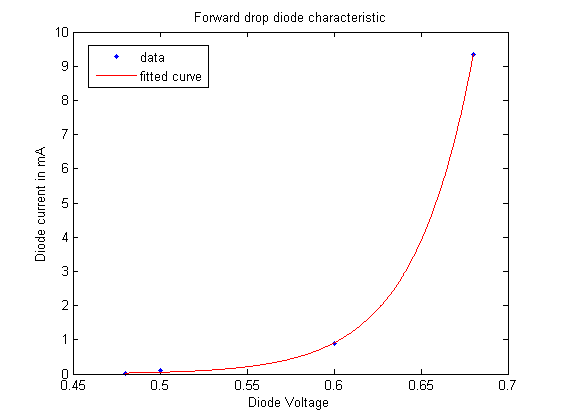
\includegraphics[scale=.5]{pic1}
\captionof{figure}{Forward drop characteristic of diode from circuit configuration in figure 1}
\end{figure}

The estimate for the incremental resistance for operating current values of 0.1\si{\milli\ampere} and 10\si{\micro\ampere} are 0.512\si{\ohm} and 0.918\si{\ohm}, respectively. Using the same method of calculation, the incremental resistance of the diode at operating currents 5\si{\milli\ampere} and 0.5\si{\milli\ampere} are 4.81\si{\ohm} and 0.512\si{\ohm}, respectively.


\subsection{Small Signal Analysis}
Results not obtained.


\end{document}